\fs{whole section probably needs to fit in max 2 pages}

\sys{}'s execution protocol has three goals: 1) to offer clients an interactive transaction interface \fs{too obvious?}, 2) to be scalable, and 3) to maintain independent operability \fs{and Byzantine independence, Serializability}.

\sys{} achieves these goals by combining optimistic client-side execution with an aggressive, but Byzantine resilient, concurrency control (CC) scheme that maintains Byz-Serializability. 
\iffalse
 \la{We seem to have already made this points in the intro tio the section} \changebars{}{\sys leaves clients responsible for executing the transactions they submit, and allows every client, in parallel, to execute arbitrary interactive transactions using read RPC's, instead of submitting stored procedured that must be ordered and executed by replica servers.}  
 \fi By relying on optimistic rather than pessimistic CC schemes such as 2-phase-locking (2PL), \sys{} forgoes costly coordination to acquire locks, and sidesteps the concern of Byzantine clients refusing to relinquish locks.

\iffalse
\la{I would just remove the following} 
\changebars{}{Before we detail Indicus’s transaction processing and validation mechanism, we first discuss the CC that Indicus imple- ments as the latter are functions of the precise CC requirements.}
\fi

\subsection{\sys{}'s Concurrency Control}

%%% Explain MVTSO itself only briefly. Then explain how we make it for for byz
% 1) bound timestamps, 2) make writes visible late only, 3) only allow f+1 matchin uncommitted writes, 4) read timestamps
%Afterwards: explain execution interface. After that explain validation check. Then have overarching example
\iffalse
% we need to change a few things:
% 0) timestmap bound
% 1) Read validity
% 2) deferred writes
% 3) read uncommitted
% 4) byz read timestamps (read lock implies you had access control, at that point it is no different than issuing a tx and completing. But we do not want to give the power to abort for no reason. It should be traceable.
\fi

\fs{fig doesnt make so much sense before reading the whole thing} \fs{cut this preamble?}
Figure \ref{fig:MVTSOEX} shows an example trace of \sys operational behaviors under different request processing orders (assume $f=1$) that we use to guide the remaining outline.

\begin{figure*}
\begin{center}
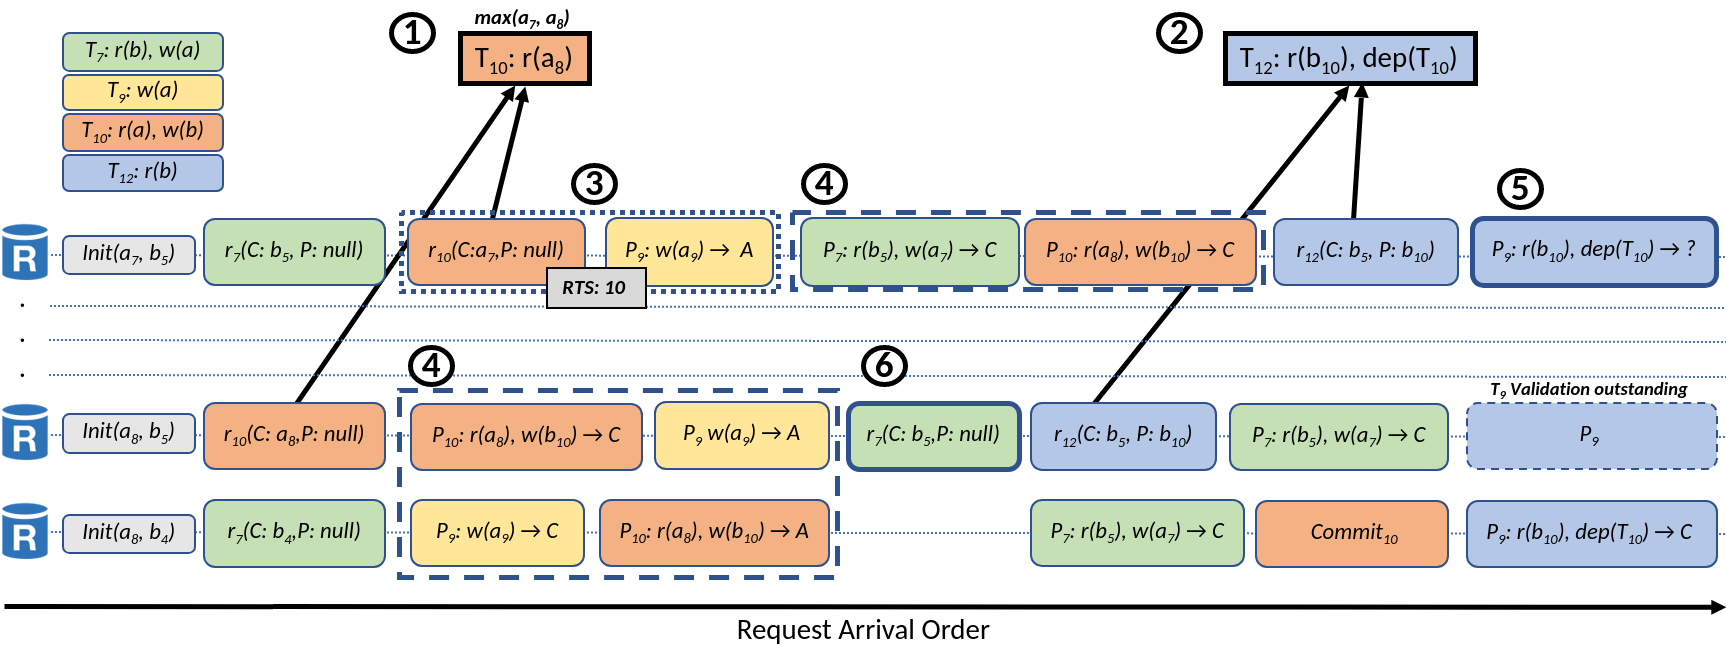
\includegraphics[width= \textwidth]{./figures/MVTSOLargeFont.png}
\end{center}
\caption{\emph{MVTSO behavior for different replica processing orders}. $r_x(C : a_y ,P : a_z)$ denotes that transaction $T_x$ (x being the timestamp of a transaction in this example) reads the version $y$ of object a written by committed transaction $T_y$ and version $z$ from tentative prepared transaction $T_z$. $P_x(RS,WS,DEP)$ denotes a transaction $T_x$'s prepare request (i.e. the validation check) for respective ReadSet (RS), WriteSet (WS) and Dependenc Set (DEP), and $\rightarrow C / A$ denotes the local replica validation outcome (Commit/Abort).} 
\label{fig:MVTSOEX}
\end{figure*}

\par \textbf{MVTSO.} Our starting point is Multiversioned Timestamp Ordering (MVTSO), a concurrency control scheme that prescribes a serialization order by assigning a speculative timestamp \textit{before} execution \cite{bernstein1983multiversion, reed1983implementing, su2017tebaldi}. In MVTSO, reading object $o$  returns $o$'s  the latest written version smaller than the readers' timestamps. A writer attempting to create a new version of $o$  must abort if a higher timestamped read has already retrieved an earlier version (if it didn't, that read operation would appear to have ``missed a write''). A transaction may commit only if all read-write dependencies have committed.

\iffalse
\fs{cut the whole following paragraph?} \la{Yes, I would cut it} This allows us to a) only classify concurent read/write operations as conflicting if their execution results violate the timestamp order (Fig. \ref{fig:MVTSOEX}: 4 bottom), and b) avoid write/write conflicts alltogether. 
When speculative execution results match the pre-defined timestamp order, no aborts are necessary (Fig. \ref{fig:MVTSOEX}: 4 top). \sys{}'s challenge is therefore to a) assign appropriate timestamps and b) coordinate execution in a way that maximizes such coherence; the presence of Byzantine participants (clients/replicas) complicates this.

In MVTSO, reads operations return the latest written version smaller than the readers' timestamps, while writers attempt to create new versions at their timestamp, but must abort if a higher timestamped read would have "missed the write" by reading a prior version. A transaction may commit only, if all read-write dependencies have committed.
\fi

When \sys{}'s speculative execution results match the pre-defined timestamp order, no aborts are necessary (Fig. \ref{fig:MVTSOEX}: 4). \sys{}'s challenge is therefore to a) assign appropriate timestamps and b) coordinate execution in a way that maximizes such coherence; the presence of Byzantine participants (clients/replicas) complicates this.

\par \textbf{Byzantine resilience.} Read operations in \sys have the following sub-goals: \one Correct clients should read valid data, i.e. experience read integrity, \two Correct clients should read fresh data, i.e. minimize staleness and hence maximize commit chance, and \three Reads must provide the context necessary to potentially complete observed write state. 
Clients validate the integrity of reads by requiring replicas to provide a proof of validity, which consists of a set of signatures confirming committment, or if not yet existant, a set of  $f+1$ replica's tentative commit endorsements \fs{maybe cut this second part, since it will become redundant}. Moreover, to guarantee that clients do not read maliciously stale data from their local replica, \sys encourages clients to read the latest version across $\geq f+1$ replicas (Fig. \ref{fig:MVTSOEX}: 1,2).
Avoiding Byzantine influence comes at a cost: Read operations require a synchronous, potentially WAN \fs{or just remote - i.e. not local}, rountrip. 

MVTSO intuitively synergizes well with \sys{}'s potenially WAN remote reads as reading from a fixed timestamp helps speculative readers observe consistent snapshots, even when execution is long and consequently interleavings are frequent (Fig. \ref{fig:MVTSOEX}: 6). \fs{at the price of experiencing serializability instead of strict serializability - that is only the case if your timestamps are outdated}.

While we assume that clocks are loosely synchronized across correct participants, Byzantine participants may diverge arbitrarily and propose excessively high timestamps. A simple solution is to bound time-stamps by querying the median time from a Quorum of replicas and including replies as proof \cite{bazzi2004non, bazzi2018clairvoyant}. To side-step the additional overheadd that a dedicated timestamping phase incurs, we compromise by allowing clients to optimistically select their own timestamps, but reject request timestamps above a threshold at all correct replicas, thus incentivising clients to select bounded, close to real-time, timestamps. 

In traditional MVTSO, writes become visible to successive, higher timestamped, reads immediately. However, in the presence of Byzantine clients this is undesirable, as it allows clients to issue write operations without the intention of ever committing a transaction. Thus, any correct clients' read that observes, and consequently depends on a Byzantine clients write may be blocked indefinitely.
%Allowing other clients to preemtively commit outstanding write operations is infeasible, as the remaining transaction procedure is known only to the issuing client, while conceiding pessimistic abort permission empowers Byzantine participants to obstruct any correct clients' writes. 
\sys reconciles this dilemma by deferring all database updates until execution is complete and the client prepares the transaction for commitment. 
% Concretely, \sys clients buffer all write operations, and submit them only when attempting to commit the transaction, thereby enabling other \sys client to orderly complete Validation and Writeback steps.\\
\la{This needs to be better explained} \fs{took a pass:}
Clients in \sys distinguish explicitly between writes \textit{committed} across all involved shards and tentative writes \textit{prepared} at a single shard: While clients accept all verifiable \textit{committed} version from a single replica, they accept \textit{prepared} versions only when endorsed by $f+1$ replicas. This ensures that a) at least one correct replica believes that the write can commit, and hence is worth observing, and b) that Byzantine replicas and clients cannot collude to violate Byzantine independence by reactively inventing versions. \fs{such invented transactions could be designed to be guaranteed to abort: I.e. by claiming to have read an out-dated version. The write versions could be engineered to be perfectly at the bound of the read timestamp, such that it is guaranteed to be chosen}\\
Finally, \sys replicas evaluate writes for conflicts by maintaining a Read Timestamps (RTS) for each locally processed read (Fig. \ref{fig:MVTSOEX}: 3). While this allows un-prepared reads to elicit external effects, these affect only concurrent transactions with smaller timestamps and can be bypassed by re-trying a transaction. To nonetheless limit recurrent abuse, we discuss a personalized lease mechanism to limit Byzantine influence in section Y.z (Optional Modifc). \fs{or just do it here in 1-2 sentences. We do not implement this though.}



\subsection{Execution interface}
Client applications execute transactions via the following interface. A TX object \textit{TXObj $\coloneqq$ (SeqNo, ClientID, InvolvedShards, ReadSet, WriteSet, Dependencies)}, records the state necessary for Validation.

\iffalse
\begin{figure}
\begin{center}
\includegraphics[width= 0.5\textwidth]{./figures/TxState.png}
\end{center}
\caption{Transaction execution state}
\label{fig:Txstate}
\end{figure}
\fi

\textbf{Begin()} A client begins a transaction by optimistically choosing a timestamp \textit{TS $\coloneqq$ (Time, ClientID)} that defines a total serialization order across all clients.  \\
\textbf{Write(key, value)}. A client buffers the write: \textit{WriteSet = WriteSet $\cup$ (key, value)}\\
%%%%%%%%%Read protocol%%%%%%%%%%%
\textbf{Read(key, TS, RQS)} 
If \textit{key $\in$ WriteSet} a client returns the buffered write value. Otherwise, the client conducts a remote read for given hyperparameter Read Quorum Size (RQS):

\fbox{\begin{minipage}{23em}

\textbf{1: C} $\rightarrow$ \textbf{R}: Client sends read request to Replicas
\end{minipage}}\\
%Improve RQS formulation
A client broadcasts a read request  $m = (Read, key, TS)_c$.
\iffalse
 to $RQS$ different replicas. Note, that in order to guarantee $\geq RQS$ replies a client might need to send up to $f$ additional requests to compensate for unresponsive/faulty participants ($max(|Replies|) \leq n-f$). 
\fi
\fs{Optimization: A client sends only to RQS+f to receive RQS many replies}

\fbox{\begin{minipage}{23em}
\textbf{2: R} $\rightarrow$ \textbf{C}: Replica processes client read and replies
\end{minipage}}\\
A replica authenticates the client\footnote{Byzantine replica may ignore read access control. Solving this problem is beyond the scope of this work; we defer to existing solutions \cite{basu2019efficient}.}, and enforces a local timestamp threshold. \fs{this can probably be shortened:} It returns a signed message \text{$\langle \textit{ReadReply, Committed, Prepared} \rangle _R$}, where $Committed \coloneqq (value, version, proof)$ represents the value-version pair with largest committed write version smaller than TS and a proof of commitment,  and $Prepared \coloneqq (value, version, TxID', deps)$ the respective largest uncommitted value-version pair, the associated transaction ID, and the latter transactions potentially uncommitted read-write dependencies. Moreover, a Replica stores a new read timestamp (RTS) for the key: $RTS(key) = RTS(key) \cup TS$ (Fig. \ref{fig:MVTSOEX}: 3). 
\fs{a replica may include a set of prepared values to increase likelihood of client receiving f+1 matching}

\fbox{\begin{minipage}{23em}
\textbf{3: C} ($\rightarrow$ \textbf{R}): Client receives read replies 
\end{minipage}}\\
A client waits for $\geq RQS$ read replies and chooses the biggest valid result \textit{(value, version) $= max_{valid}$(\{Committed\},\{Prepared\}} (Figure \ref{fig:MVTSOEX}: 1,2). A \textit{Committed} tuple is valid, if the proof confirms commitment, wheras a \textit{Prepared} is valid iff there exist $f+1$ matching \textit{Prepared$_r$}. The client adds the version to its read set \textit{ReadSet = ReadSet $\cup$ (key, version)} and additionally claims a dependency if it was a \textit{Prepared} version: \textit{Dep = Dep $\cup$ \{f+1 $\times$ Prepared$_r$ \}} . 

\fs{la: finds the use of commit in both exec and validation confusing. Is it unclear that this refers to application here?}
\textbf{Commit()} A Client terminates its execution, and computes a unique transaction identifier based on final execution object and its timestamp: $TxID \coloneqq (H(TxObj, TS)$, thus preculding Byzantine participants from equivocating transaction contents. It then initiates the Validation Phase by issuing a 2PC-Prepare requests to each involved shard.
%What if a byz doesnt send to all involved shards? It will be visible on some shard and hence an correct client can obtain the full TX. See Hierarchical IDS in Protocol.tex

\textbf{Abort()} A client terminates execution, and broadcasts a request to release all acquired Read Timestamps (RTS). Since writes in \sys are deferred, no other rollback action is necessary.


We briefly discuss some implications of the choice of Read Quorum Size (RQS). Following cases may be distinguished: \one \textbf{$RQS = 1$} A client may read committed data from just \textit{trusted} replica (at the risk of reading stale data) to reduce execution latency and consequently minimize conflicting interleavings. \two \textbf{$RQS \geq f+1$} \sys{}'s recommended minimal mode of operation. While side-stepping maliciously stale reads, it is still possible to read (arbitrarily) stale data due to replica inconsistency, caused by either asynchrony or partial transaction replication by a Byzantine client.
\three \textbf{$RQS \geq \frac{n+f+1}{2}$} When reading from a Quorum of sufficient size to overlap with any Validation Quorum (ref section Validation) in at least one correct replica, a client guarantees, that no more \textbf{additional} (beyond previously observed) conflicting writes can be admitted, since such a Quorum of acquired RTS acts as a read-lock. 

\iffalse
Trusting only $f+1$ matching prepared writes has the beneficiary side effect of allowing us to include only transaction identifiers as dependencies, rather than the full transaction, since it is guaranteed that at least one correct replica has stored the transaction. Thus, in the failure free scenario, where clients need not complete transactions $in Dep$, \sys minimizes the meta-data overhead that the recovery protocol imposes.
\fi

We remark that, consistent with Byz-Isolation, \sys allows Byzantine clients to fabricate and (permissibly) submit arbitrary reads; Byzantine clients may \textit{choose} whether to read legal, or even real data.  \sys does, however, enforce that Byzantine clients cannot (undetectably) fabricate dependencies by requiring a proof of $f+1$ matching prepared writes. This precludes Byzantine clients from indetectibly stalling their own transactions and consequently obstructing liveness for consecutive descendant (second degree...) dependencies.
Furthermore, this allows \sys to include only transaction identifiers as dependencies, rather than the full transaction, thereby minimizing the common path overhead. The full transaction can be acquired from an correct replica when necessary. We discuss how to complete stalled or slow transactions in section Y (Granting Liveness).




